\subsection{Inter-module flows}
The figures ~\ref{fig:Case1Modules}, ~\ref{fig:Case2Modules},~\ref{fig:Case3Modules} and ~\ref{fig:Case4Modules} show an extract of the data and event flow between modules in the four cases we have been examining. The most prominent flows data-wise are indicated in red arrows, followed by black arrows for less prominent data flows and green for flows that are negligible in data flow but not in event count. Solid arrows indicate a prominence in the number of data events, followed by dashed arrows for less prominent event flows and dotted arrows for flows that are
negligible in event flow but not in data flow. Flows that are both negligible in data-flow and event flow are not displayed to keep the figures from becoming to filled with irrelevant information for the case at hand. Note that modules as data producer are denoted using a square box while (possibly the same) modules in their role in their role as data consumer are denoted with an oval shape. Even though there are important differences due to the differences in types of and size of investigations, we do also see a few clear similarities in these flows. To emphasize these similarities, ~\ref{fig:RoughModules} on page ~\pageref{fig:RoughModules} shows these same pictures using a grouping of modules that play a less prominent role in the analysis of the flows. Below we summarize the core information that we can conclude from these four condensed figures:
\begin{enumerate}
\item The majority of all data (roughly between 80\% and 95\%) is forwarded by the kickstart functionality to the carver functionality and never passes the digest checking module.
\item The majority of evidence data checked by the digest check module originates from either the carver or the kickstarting functionality.
\item About one third to half of the data sent to the digest check module originates from the carver, about 50\% to 60\% from the kickstart functionality.
\item Only roughly 1\% to 15\% of evidence data sent to the digest check module ends up matching. The remaining data is forwarded to the file-type check module.
\item Only roughly 15\% to 35\% of data forwarded to the file-type check module ends up being forwarded for processing any further.
\end{enumerate} 
This information, combined with what we have seen in our earlier analysis�es allows us to draw some important conclusions that we shall discuss in the following sections of this appendix.
\begin{figure}
  \centering
  \includegraphics[width=130mm]{ocfa/step5/stripped1_modules.eps}
  \caption{Case 1 inter-module flows}
  \label{fig:Case1Modules}
\end{figure}
\begin{figure}
  \centering
  \includegraphics[width=130mm]{ocfa/step5/stripped2_modules.eps}
  \caption{Case 2 inter-module flows}
  \label{fig:Case2Modules}
\end{figure}
\begin{figure}
  \centering
  \includegraphics[width=130mm]{ocfa/step5/stripped3_modules.eps}
  \caption{Case 3 inter-module flows}
  \label{fig:Case3Modules}
\end{figure}
\begin{figure}
  \centering
  \includegraphics[width=130mm]{ocfa/step5/stripped4_modules.eps}
  \caption{Case 4 inter-module flows}
  \label{fig:Case4Modules}
\end{figure}
\begin{figure}
\centering
\subfloat[case 1]{
  \includegraphics[width=60mm]{ocfa/step5/stripped1_modtypes.eps}
}
\subfloat[case 2]{
  \includegraphics[width=60mm]{ocfa/step5/stripped2_modtypes.eps}
}
\hspace{0mm}
\subfloat[case 3]{
  \includegraphics[width=60mm]{ocfa/step5/stripped3_modtypes.eps}
}
\subfloat[case 4]{
  \includegraphics[width=60mm]{ocfa/step5/stripped4_modtypes.eps}
}
\caption{Rough data flow}
\label{fig:RoughModules}
\end{figure}
